\documentclass[xcolor=pdftex,x11names,table,hyperref]{beamer}

\usepackage{verbatim}
\usepackage{setspace}
\usepackage{amsmath}
\usepackage{url}
\usepackage{xcolor} % See documentation PDF at http://www.ctan.org/pkg/xcolor
\definecolor{darkgreen}{rgb}{0,0.3,0}
\definecolor{darkblue}{rgb}{.05,.05,.30}
\definecolor{lightgrey}{rgb}{0.65,0.65,0.65}
\usepackage{tikzsymbols}


\setbeamertemplate{section in toc}[sections numbered]
\setbeamertemplate{subsection in toc}[subsections numbered]
\setbeamertemplate{subsubsection in toc}[subsubsections numbered]
\usetheme{Singapore}
\setbeamertemplate{navigation symbols}{}
\setbeamertemplate{footline}{%
\vspace{0.0em}%
\hspace{0.5em}%
{\color[rgb]{.1,.1,.1} \insertframenumber{}~/~\inserttotalframenumber}
}

\newcommand{\code}[1]{{\color{darkgreen}\texttt{#1}}}
\newcommand{\detail}[1]{{\color{lightgrey}\small{}#1}}
\newcommand{\teeny}[1]{\scalebox{0.09}{#1}}
\newcommand{\tablecolors}{\rowcolors{2}{blue!12}{white}} % Cool table colors


\begin{document}

\title{Log-linear Models \\[1.5em]
 %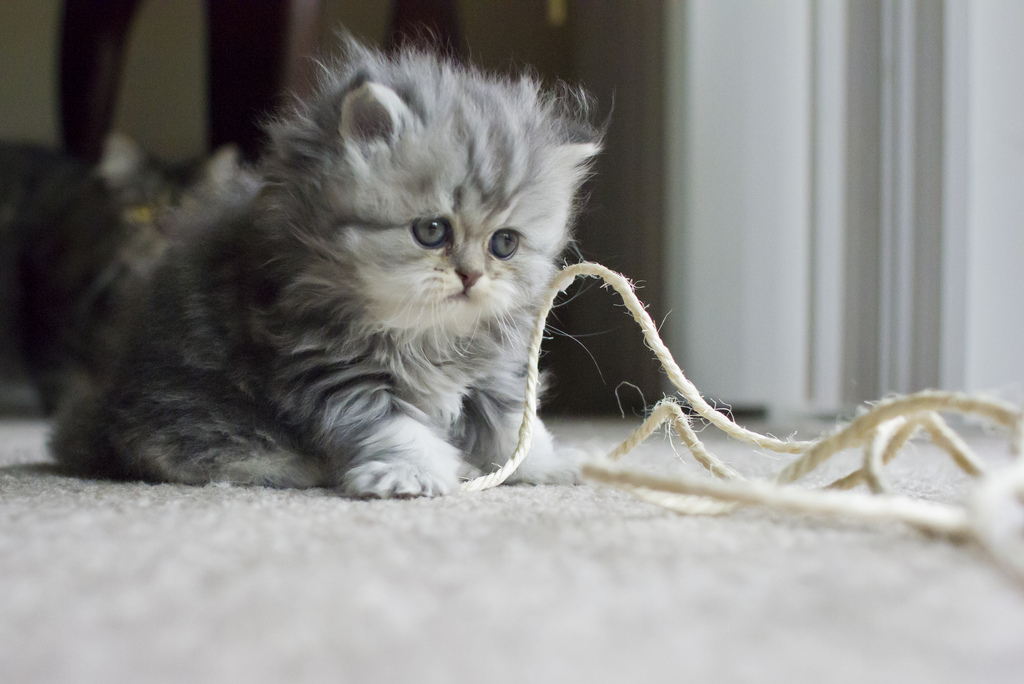
\includegraphics[width=0.5\textwidth]{images/kitten_string_flickr_albaraa.jpg} \\[-1.0em]
 %\small{Possibilities} \\[1.0em]
 %LT1 \\[1.0em]
 }
\author{\href{http://jon.dehdari.org}{Jon Dehdari}}
\frame{\titlepage}

\begin{frame}{Good Morning!}
	\begin{center}
	%\includegraphics[width=0.8\textwidth]{images/.jpg}
	\end{center}
\end{frame}

\begin{frame}{Some Preliminaries}
\begin{description}
	\item[Vector]: In this context, a sequence of numbers. Eg.:
	\begin{equation*}
	{\bf x} = \overrightarrow{x} = \langle 2.1, \, -8.5, \, 0.1 \rangle
	\end{equation*}
	\pause
	\item[Dot Product]: Multiplying corresponding elements of two vectors, then adding them all up (here, a.k.a.\ `inner product')
	\begin{equation*}
	{\bf x \cdot y} = {\bf x^Ty} =  \sum_{i=1}^n x_i \times y_i = x_1 \, y_1 + x_2 \, y_2 + x_3 \, y_3 \ldots
	\end{equation*}
\end{description}
\end{frame}

\begin{frame}{Some Preliminaries}
\begin{description}
	\item[Euler's Number]: $e \, = 1 + \frac{1}{1} + \frac{1}{1\cdot 2} + \frac{1}{1\cdot 2\cdot 3} + \cdots \, \approx {\bf 2.71828} $
	\pause
	\item[Matrix]: A 2-dimensional vector
	\begin{equation*}
	{\boldsymbol A} =
	\begin{bmatrix}
	2.1 & -8.5 & 0.1 \\
	1.1 & 5.0 & -4.4
	 \end{bmatrix}
	\end{equation*}
	\pause
	\item[Tensor]: In this context, an $n$-dimensional vector
\end{description}
\end{frame}

%\begin{frame}{Log-linear Models}
\begin{frame}[fragile]\frametitle{Log-linear Models}
	\begin{Large}
	\begin{align}
	%\hspace*{-5.5em}%
		P(y | \mathbf{x}) & = \frac{e^{\boldsymbol W_y \cdot \mathbf{x}} }{Z} \hspace*{0.4em} \substack{\color{green}{ \leftarrow \, \text{\parbox[c]{0.55\textwidth}{ {\tiny \, exponentiation helps ensure scores are positive}}}} \\[1.0em]  \color{green}{ \leftarrow \, \text{\parbox[c]{0.55\textwidth}{ \textbf{normalization constant}, {\footnotesize to ensure the \\[-0.9em] prob.\ of all possible outcomes sums to 1}}}}}  \nonumber\\[1.0em]
							%& = \frac{1}{Z} e^{\boldsymbol W_y \cdot \mathbf{x}}  \nonumber\\[1.0em]
							& =	\frac{e^{\boldsymbol W_y \cdot \mathbf{x}}}{\sum_h e^{\boldsymbol W_h \cdot \mathbf{x}}}  \,\, \substack{ \, \\[1.0em]  \color{green}{ \leftarrow \text{\parbox[c]{0.50\textwidth}{ \, to get Z, we just add up scores from \\[-0.8em] all possible outcomes}}}} \nonumber\\[1.0em]
							& = \text{softmax}(\boldsymbol W_y \cdot \mathbf{x}) \nonumber%\\[1.0em]
							%& =  \nonumber\\[1.0em]
	\end{align}
	\end{Large}
	\pause

	The input vector $\bf x$ includes an additional dummy value of 1.0\,, called a \textbf{bias term}.
	This helps determine the offset of the linear separator.  % (but not the shape, for nn's)
\end{frame}


\begin{frame}{Finding Good Values for $\bf W$}
	\begin{center}
	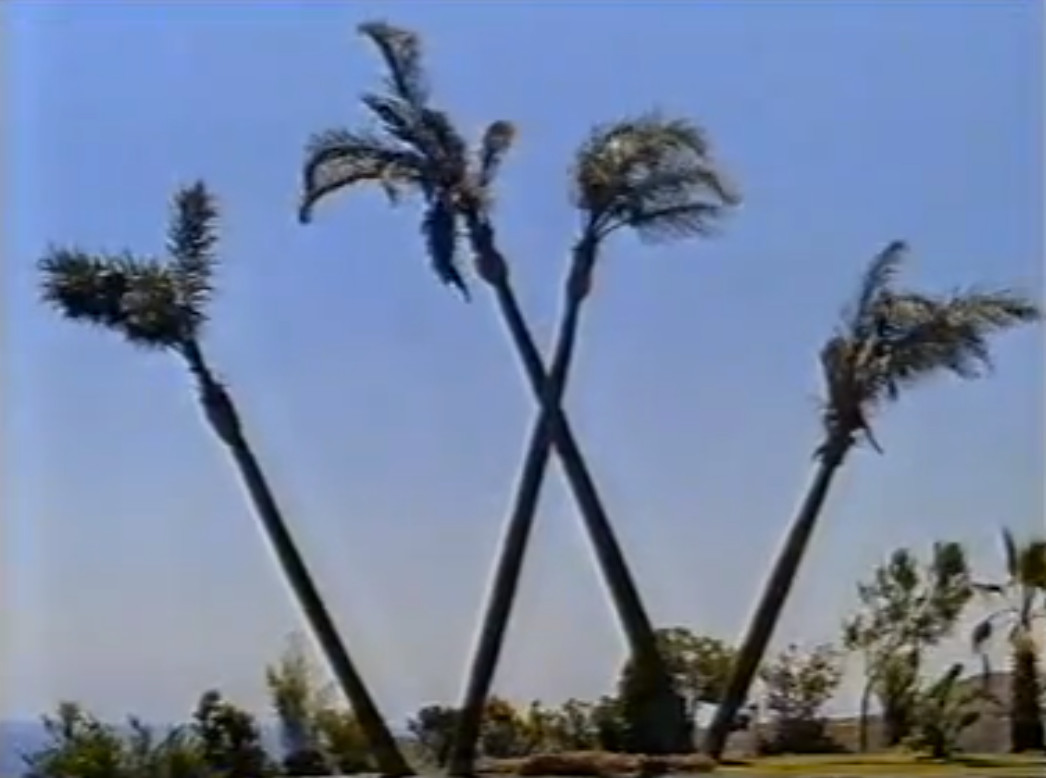
\includegraphics[width=0.36\textwidth]{images/big-w.jpg}
	\end{center}
\begin{itemize}
	\item The weight matrix $\bf W$ constitutes the \textbf{parameters} of the model
	\item Then the main task is to find good values for the weight matrix $\bf W$
	\item This is done by common \textbf{optimization} techniques, like \href{https://en.wikipedia.org/wiki/Limited-memory_BFGS}{L-BFGS}
\end{itemize}
\end{frame}

\begin{frame}{}
\begin{itemize}
	\item 
	\item 
\end{itemize}
\end{frame}




% \begin{frame}{}
% \begin{block}{}
% \begin{itemize}
% 	\item 
% 	\item 
% 	\item 
% \end{itemize}
% \end{block}
% \end{frame}


\end{document}
